	\documentclass[10pt]{article}
\usepackage{graphicx}
\usepackage{float}
\usepackage{amsmath}
\usepackage[margin=0.7in]{geometry}
\usepackage{caption}
\usepackage{subcaption}
\usepackage{multicol}

\restylefloat{figure}
	\title{IT3708 - Exercise 3}
\author{
        Eirik Hammerstad \& Nicklas Utgaard
}
				
\date{\today}
\begin{document}
\maketitle
%\pagebreak
%\tableofcontents
%\pagebreak
\section{Overview}
	\subsection{System}
		The system used to solve this exercise consists of four maven projects\footnote{Maven - http://maven.apache.org/}, 
		\begin{table}[H]
			\begin{tabular}{ll}
				\textbf{GA} & Genetic algoritm framework\\
				\textbf{ANN} & Artificial neural network framework\\
				\textbf{TrackerGame} & TrackerGame implementation and APIs\\
				\textbf{CTRNNBundle} & The exercise specific classes, and bundling of all dependencies.
			\end{tabular}
			\caption{The overall structure for this exercise can be seen in figure~\ref{fig:struct}.}
			\label{tabel:project}
		\end{table}
The architecture for GA has been covered in previous deliveries in this course, and will therefor not be covered here. We will however give a brief introduction to the new projects within this exercise. 
		
	\textbf{ANN}(Figure~\ref{fig:annstruct}) gives the basis building blocks for building artificial neural networks, it is large based around the same structure one would see in graph problems\footnote{Graph theory - http://en.wikipedia.org/wiki/Graph\_theory}, but with the addition of \textit{NeuralLayer}. In comparison to normal graphs the nodes has been replaces by neurons and the edges replace by synapses. Though the \textit{NeualLayer} abstraction is not necessary it provides and easy way of structuring the network. To bring it all together and keep track of the network we have \textit{StructuredANN}.

		\textbf{TrackerGame}(Figure~\ref{fig:trackergamestruct}) is the implementation of the game described in the exercise description. It consist only of two entities, \textit{World} and \textit{TrackController}. \textit{World} is the govering entity, in charge of updating the models, and asking the \textit{TrackController} for its next move. 

		\textbf{CTRNNBundle} is the project that combines all the project into one runnable project and makes the exercise specifics implementations needed for the evolutionary algorithm (genotype, phenotype, population creator, fitnesshandler, plotting ect.). The most interesting classes in this project is \textit{ANNBuilder} and \textit{ANNTrackerController}. \textit{ANNBuilder} is the class in charge of converting the parameter array evolved into a working artificial neural network. \textit{ANNTrackerController} is a supporting class for the fitnesshandler, and preforms the simulation of the game with a neural network as the controller in order to determind the fitness of the  neural network parameters. The genotype and phenotype implementations is discussed in the next section. 
		
	\begin{figure}
		\centering
		\begin{subfigure}{.3\textwidth}
			\centering
			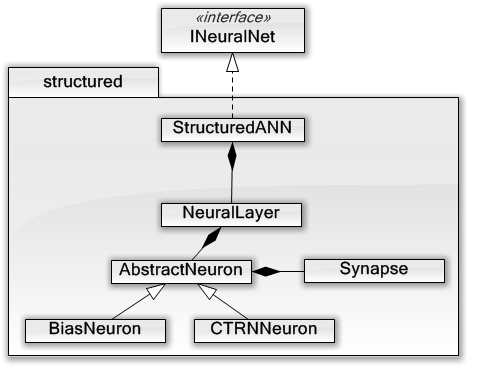
\includegraphics[width=\linewidth]{./../images/ANN.png}
			\caption{ANN structure}
			\label{fig:annstruct}
		\end{subfigure}
		\begin{subfigure}{.3\textwidth}
			\centering
			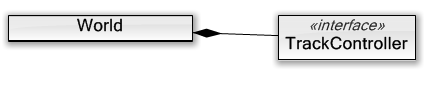
\includegraphics[width=\linewidth]{./../images/TrackerGame.png}
			\caption{TrackerGame structure}
			\label{fig:trackergamestruct}
		\end{subfigure}
		\begin{subfigure}{.3\textwidth}
			\centering
			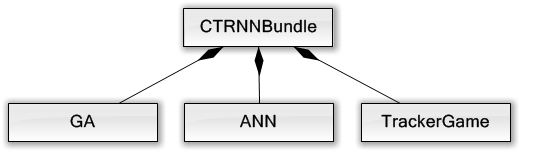
\includegraphics[width=\linewidth]{./../images/Structure.png}
			\caption{Project structure}
			\label{fig:struct}
		\end{subfigure}
	\end{figure}

	\subsection{Genotype}
		We chose a binary representation of our genotype with 8 bit accuracy. This representation is extremely similar to the one used in the previous exercise. The only big difference is the shear number of parameters (5 in previous exercise. 34 in this one, 26 weights, 4 gains, 4, time constants), which results in a much larger bitvector (272 bits). The transformation from binary to real values is however the same. 
	\begin{table}[H]
		\parbox{.45\linewidth}{
			\centering
			\begin{tabular}{ll}
				0..4 & gains for hidden then output\\
        4..8 & time constants for hidden then output\\
        8..18 & weights originating in inputlayer\\
				18..26 & weights originating in hiddenLayer\\
        26..30 & weights originating in outputlayer\\
				30..34 & weights originating in baislayer
			\end{tabular}
			\caption{Structure of bitvector}
		}
		\hfill
		\parbox{.45\linewidth}{
			\centering
			\begin{align}
				param &\in \{p_1, p_2, \dots, p_n\}\nonumber\\
				acc &= 8\nonumber\\
				bitvector &= 00001101\dots11100110\nonumber\\
				bitvector_{param} &= subvector(bitvector, param)\nonumber\\
				coef_{param} &= (bitvector_{param})_{10}\nonumber\\
				step_{param} &= (max_{param}-min_{param})/2^{acc}\nonumber\\
				param &= min_{param}+(coef_{param}*step_{param})\nonumber
			\end{align}
			\caption{Bitvector conversion}
		}
	\end{table}
	
	\subsection{Parameters}
		\begin{table}[H]
			\parbox{.45\linewidth}{
				\centering
				\begin{tabular}{ll}
					Adult selection protocol & Generational mixing\\
					Parent selection mechanism & Sigma scaling\\
					Population size & 100\\
					Number of generations & 1000\\
					Crossover rate & 0.9\\
					Mutation rate & 0.1
				\end{tabular}
				\caption{Evolution algorithm parameters}
			}
			\hfill
			\parbox{.45\linewidth}{
				\centering
				\begin{tabular}{ll}
					Tracker size & 5\\
					Object size & [1, 6]\\
					Arena size & 30 x 15\\
					Tracker speed & [-4, 4]\\
					Capture ratio & 1.0\\
					Avoidance ratio & 0.0
				\end{tabular}
				\caption{Tracker scenario parameters}
			}
		\end{table}
\section{Verification}
	We used a score based fitness function related to the number of shadows registered and the size of the object. In addition to fitness gained by catching or avoiding object, we rewarded fitness based on the speed. This was done to make an incentive to utilize speed and therefore increase the probability of reaching an object in time. The reward for catching or avoiding an object was calculated each time an object reached the bottom of the arena, while the speed reward was accumulated at each time step based on the reaction of the tracker. The basic formula for out fitness is as show below, with the different rewards varying depending on our goal.
	\begin{align}
		fitness &= \alpha catch\_reward+\beta avoid\_reward+\theta speed\_reward\nonumber\\
		ratio(shadows, size) &= \frac{shadows}{size}\nonumber
	\end{align}
In order to gauge the outcome when an object reached the bottom we use the ratio shown above.
	\subsection{Catch all}
		\subsubsection{Fitness function}
			\begin{align}
				catch\_reward(shadows, size) &= \left\{ 
				\begin{array}{l l}
					2 &\text{if $ratio=1$ and $object\_size <= 5$} \\
					2 &\text{if $ratio>0.8$ and $object\_size = 6$}\\
					0 &\text{else}
       \end{array} \right.\nonumber\\
				avoid\_reward(shadows, size) &= 0\nonumber\\
				speed\_reward(speed) &= \left\{ 
				\begin{array}{l l}
					0.000 &\text{if $|speed| < 2$} \\
					0.003 &\text{if $|speed| = 2$} \\
					0.006 &\text{if $|speed| = 3$} \\
					0.009 &\text{if $|speed| = 4$} \\
       \end{array} \right.\nonumber\\
			 \alpha =\beta =\theta &= 1\nonumber\\
			\end{align}
		\subsubsection{Parameters}
		\subsubsection{Results}
	\subsection{Catch and avoid}
		\subsubsection{Fitness function}
		\subsubsection{Result}
\section{Modified tracker scenario}
\section{Modified topology}
\section{Modified variable ranges}
\section{In depth}
\section{Appendix}
	
\end{document}